\documentclass{article}
\usepackage{moon}

\usepackage[some,center]{background}
\backgroundsetup{
scale=1,
%color=black,
opacity=1,
angle=0,
contents={%
  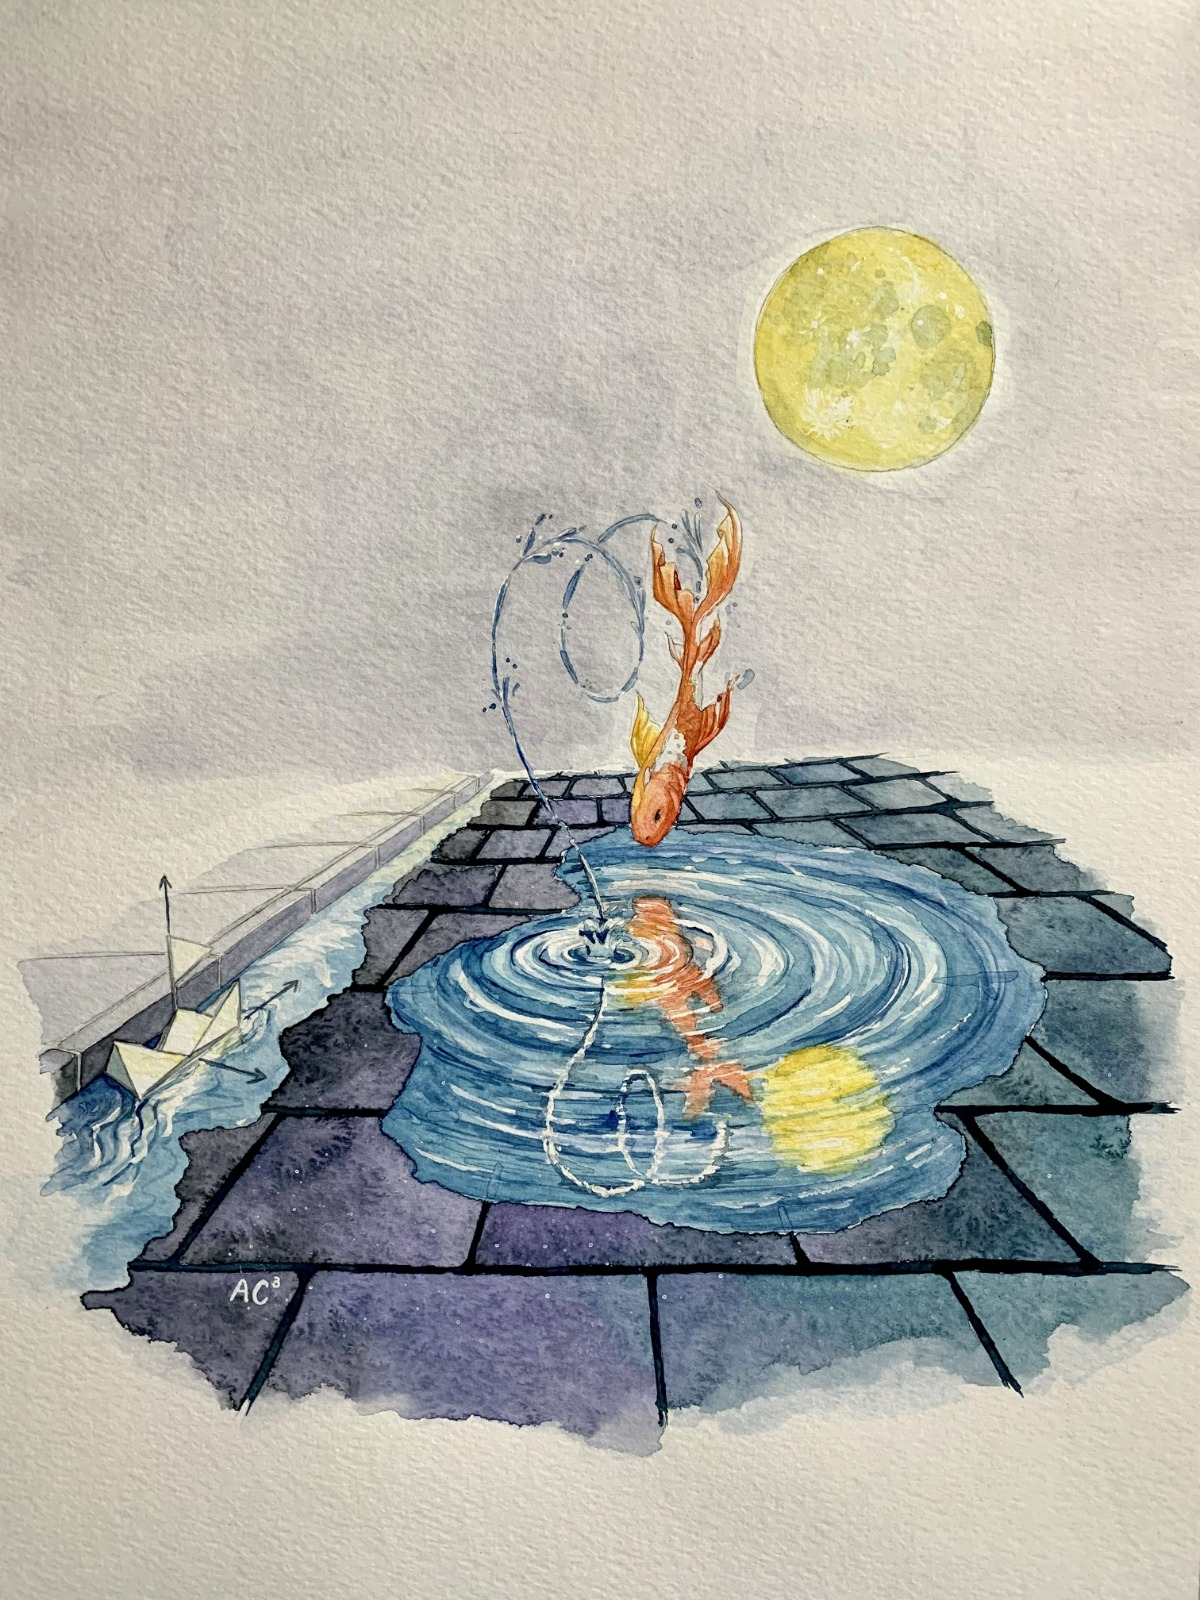
\includegraphics[width=\paperwidth%,height=\paperheight
  ]{jpg/Moon}
  }%
}

\hypersetup{pdftitle={Moon in a puddle and four-vertex theorem},
pdfauthor={Anton Petrunin and Sergio Zamora Barrera with artwork by Ana Chávez Cáliz}}


\begin{document}
%\pagestyle{empty}

\BgThispage

\title{Moon in a puddle and the four-vertex theorem}
\author{%Anton Petrunin and Sergio Zamora Barrera\\ with artwork by Ana Chávez Cáliz
}
\date{}
\maketitle

\thispagestyle{empty}\newpage

The theorem about the Moon in a puddle is not very well known, but it deserves to be included in standard introductory texts on differential geometry of curves.
It gives the simplest meaningful example of a local-to-global theorem which is mainly what differential geometry is about.

This note is divided in two parts:  first --- we present a proof of the Moon in a puddle theorem, and second --- we use its key lemma to prove a generalization the well-known four-vertex theorem.


\section*{Moon in a puddle}

The following question was initially asked by Abram Fet and later solved by Vladimir Ionin and German Pestov \cite{pestov-ionin}.

\begin{thm}{Theorem}\label{thm:moon-orginal}
Assume $\gamma$ is a simple closed smooth regular plane curve with curvature bounded in absolute value by~1.
Then the region surrounded by $\gamma$ contains a unit disc.
\end{thm}


{

\begin{wrapfigure}{r}{33 mm}
\vskip-6mm
\centering
\includegraphics{mppics/pic-62}
\vskip0mm
\end{wrapfigure}

A straightforward approach would be to start with some disc in the region and blow it up to maximize its radius.
However, as one may see from the spinner-like example on the diagram, it does not always lead to a solution --- a closed plane curve of curvature at most 1 may surround a disc of radius smaller than 1 that cannot be enlarged continuously.

}

We present %the proof from our textbook \cite{petrunin-zamora} which is 
a slight improvement of the original proof.
There are other solutions: 
One is based on curve-shortening flow; it is given by Konstantin Pankrashkin  \cite{pankrashkin}.
Another use cutlocus; it is sketched in %\cite{petrunin-2020,panov-petrunin}, and 
\cite[Problem 1.7.19]{toponogov}.

Let us mention that an analogous statement for surfaces does not hold --- there is a solid body $V$ in the Euclidean space bounded by a smooth surface whose principal curvatures are bounded by 1 such that $V$ does not contain a unit ball; moreover one can assume that $V$ is homeomorphic to the 3-ball.
Such an example can be obtained by inflating a nontrivial contractible 2-complex in $\RR^3$ 
(Bing's house constructed in \cite{bing} would do the job).
This problem is discussed by Abram Fet and Vladimir Lagunov \cite{lagunov-2,lagunov-fet}%; see also our textbook \cite{petrunin-zamora}
.

\medskip

Let us use the term \emph{circline} as a shortcut for a \emph{circle or line}.
Note that the osculating circline of a smooth regular simple curve is defined at each of its points --- there is no need to assume that the curvature does not vanish.

Suppose that $\gamma$ is closed simple plane curve (simple means that it has no self-intersections).
We say that a circline $\sigma$ \emph{supports} a curve $\gamma$ at a point $p$ if the point $p$ lies on both $\sigma$ and $\gamma$, and the cicrline $\sigma$ lies in one of the closed regions that $\gamma$ cuts from the plane.
If furthermore this region is bounded, then  we say that $\sigma$ \emph{supports} $\gamma$ \emph{from inside}.
Otherwise, we say that $\sigma$ \emph{supports} $\gamma$ \emph{from outside}.



\begin{thm}{Key lemma}\label{thm:moon}
Assume $\gamma$ is a simple smooth regular plane loop.
Then at one point of $\gamma$ (distinct from its base) its osculating circle $\sigma$ %globally?
 supports $\gamma$ from inside.
\end{thm}

First let us show that the theorem follows from the lemma.

\parit{Proof of \ref{thm:moon-orginal} modulo \ref{thm:moon}.}
Since $\gamma$ has absolute curvature at most 1, each osculating circle has radius at least 1.
According to the key lemma one of the osculating circles $\sigma$ supports $\gamma$ from inside.
In this case $\sigma$ lies inside of $\gamma$, whence the result.
\qeds

\parit{Proof of \ref{thm:moon}.}
Denote by $F$ the closed region surrounded by $\gamma$.
We can assume that $F$ lies on the left from $\gamma$.
Arguing by contradiction,
assume that the osculating circle at each point $p\in \gamma$ does not lie in~$F$.

\begin{figure}[!ht]%{r}{38 mm}
\vskip-0mm
\centering
\includegraphics{mppics/pic-32}
\vskip0mm
\end{figure}

Given a point $p\in\gamma$ let us consider the maximal circle $\sigma$ that lies completely in $F$ and is tangent to $\gamma$ at $p$.
The circle $\sigma$ will be called the {}\emph{incircle} of $F$ at $p$.

Note that the curvature $\skur_\sigma$ of the incircle $\sigma$ has to be strictly larger than the signed curvature of $\gamma$ at $p$, further denoted by $\skur(p)_\gamma$.
It follows that $\sigma$ has to touch $\gamma$ at another point.
Otherwise we can increase $\sigma$ slightly while keeping it inside $F$.

Choose a point $p_1$ on $\gamma$ that is distinct from its base point, and  let $\sigma_1$ be the incircle at $p_1$.
Denote by $\gamma_1$ an arc of $\gamma$ from $p_1$ to a first point $q_1$ on $\sigma_1$.
Denote by $\hat\sigma_1$ and $\check\sigma_1$ the two arcs of $\sigma_1$ from $p_1$ to $q_1$ such that the cyclic concatenation of $\hat\sigma_1$ and $\gamma_1$ surrounds~$\check\sigma_1$.

Let $p_2$ be the midpoint of $\gamma_1$, and $\sigma_2$ be the incircle at $p_2$.

Note that $\sigma_2$ cannot intersect $\hat\sigma_1$.
Otherwise, if $\sigma_2$ intersects $\hat\sigma_1$ at some point $s$, then $\sigma_2$ must have two more common points with $\check\sigma_1$, say $x$ and $y$ --- one for each arc of $\sigma_2$ from $p_2$ to $s$.
Therefore $\sigma_1\z=\sigma_2$ since these two circles have three common points: $s$, $x$, and $y$. 
On the other hand, by construction, $p_2\in \sigma_2$ and $p_2\notin \sigma_1$ --- a contradiction.

\begin{wrapfigure}{r}{32 mm}
\vskip-5mm
\centering
\includegraphics{mppics/pic-64}
\caption*{Two ovals pretend to be circles.}
\vskip0mm
\end{wrapfigure}

Recall that $\sigma_2$ has to touch $\gamma$ at another point.
From above it follows that it cannot touch $\gamma \backslash \gamma_1$, and therefore we can choose an arc $\gamma_2\subset \gamma_1$ that runs from $p_2$ to a first point $q_2$ on $\sigma_2$.
Since $p_2$ is the midpoint of $\gamma_1$, we have that
\[\length \gamma_2< \tfrac12\cdot\length\gamma_1.\leqno({*})\]

Repeating this construction recursively,
we get an infinite sequence of arcs $\gamma_1\supset \gamma_2\supset\dots$;
by $({*})$, we also get that 
\[\length\gamma_n\to0\quad\text{as}\quad n\to\infty.\] 
Therefore the infinite intersection $\gamma_1\cap\gamma_2\cap\dots$
contains a single point; denote it by $p_\infty$.

Let $\sigma_\infty$ be the incircle at $p_\infty$; it has to touch $\gamma$ at another point, say $q_\infty$.
The same argument as above shows that $q_\infty\in\gamma_n$ for any $n$.
It follows that $q_\infty =p_\infty$ --- a contradiction.
\qeds

\begin{thm}{Exercise}\label{ex:moon-rad}
Assume that a closed smooth regular curve $\gamma$ lies in a figure $F$ bounded by a closed simple plane curve.
Suppose that $R$ is the maximal radius of a disc contained in $F$.
Show that the absolute curvature of $\gamma$ is at least $\tfrac1R$ at some parameter value.
\end{thm}


\section*{Four-vertex theorem}


The key lemma in the previous section implies a generalization of the famous four-vertex theorem stated below.

Recall that a \emph{vertex} of a smooth regular curve is defined as a critical point of its signed curvature;
in particular, any local minimum (or maximum) of the signed curvature is a vertex.
For example, every point of a circle is a vertex.

The classical four-vertex theorem says that \emph{any closed smooth regular plane curve without self-intersections has at least four vertices}.
It has a number of different proofs and generalizations.
One of our favorite proofs was given by Robert Osserman \cite{osserman}; this paper also contains a short account on the history of the theorem.

Note that if an osculating circline $\sigma$ at a point $p$ supports $\gamma$, then $p$ is a vertex.
The latter is easy to check directly, but it also follows from the Tait--Kneser spiral theorem \cite{ghys-tabachnikov-timorin}.
Therefore the following theorem is indeed a generalization of the four-vertex theorem:

\begin{thm}{Theorem}\label{thm:4-vert}
Any smooth regular simple plane curve is supported by its osculating circline at 4 distinct points; two from inside and two from outside.
\end{thm}

\begin{wrapfigure}{r}{33 mm}
\vskip-0mm
\centering
\includegraphics{mppics/pic-63}
\vskip0mm
\end{wrapfigure}

\parit{Proof.}
According to the key lemma (\ref{thm:moon}), there is a point $p\in\gamma$ such that its osculating circle supports $\gamma$ from inside.

The curve $\gamma$ can be considered as a loop with $p$ as its base.
Therefore the key lemma implies the existence of another point $q\in\gamma$ with the same property.

This shows the existence of two osculating circles that support $\gamma$ from inside;
it remains to show existence of two osculating circles that support $\gamma$ from outside.

Let us apply to $\gamma$ an inversion with respect to a circle whose center lies inside~$\gamma$.
Then the obtained curve $\gamma_1$ also has  two osculating circles that support $\gamma_1$ from inside.

Note that these osculating circlines are inverses of the osculating circlines of $\gamma$.
Indeed, the osculating circline at a point $x$ can be defined as the unique circline that has second order of contact with $\gamma$ at $x$.
It remains to note that inversion, being a local diffeomorphism away from the center of inversion, does not change the order of contact between curves.

Note that the region lying inside of $\gamma$ is mapped to the region outside of $\gamma_1$ and the other way around.
Therefore these two new circlines correspond to the osculating circlines supporting $\gamma$ from outside.
\qeds

\begin{thm}{Advanced exercise}\label{ex:curve-crosses-circle}
Suppose $\gamma$ is a closed simple smooth regular plane curve and $\sigma$ is a circle.
Assume $\gamma$ crosses $\sigma$ at the points $p_1,\dots,p_{2{\cdot} n}$ and these points appear in the same cycle order on $\gamma$ and on $\sigma$.
Show that $\gamma$ has at least $2\cdot n$ vertices.
\end{thm}


\begin{figure}[!ht]
\begin{minipage}{.48\textwidth}
\centering
\includegraphics{mppics/pic-65}
\end{minipage}\hfill
\begin{minipage}{.48\textwidth}
\centering
\includegraphics{mppics/pic-305}
\end{minipage}
\end{figure}

The order of the intersection points is important. 
An example with only 4 vertices and arbitrary many intersection points can be guessed from the diagram on the right. 



\sloppy
\printbibliography[heading=bibintoc]
\fussy

\end{document}
